\documentclass[fleqn]{article}
\usepackage[margin=1in]{geometry}
\usepackage[nodisplayskipstretch]{setspace}
\usepackage{amsmath, nccmath, bm}
\usepackage{amssymb}
\usepackage{enumitem}
\usepackage{graphicx}
\usepackage{float}

\newcommand{\zerodisplayskip}{
	\setlength{\abovedisplayskip}{0pt}%
	\setlength{\belowdisplayskip}{0pt}%
	\setlength{\abovedisplayshortskip}{0pt}%
	\setlength{\belowdisplayshortskip}{0pt}%
	\setlength{\mathindent}{0pt}}
	
\title{Homework 1}
\author{Owen Sowatzke}
\date{February 9, 2025}

\begin{document}

	\offinterlineskip
	\setlength{\lineskip}{12pt}
	\zerodisplayskip
	\maketitle
	
	\begin{enumerate}
		\item Given below is an illustrative layout of an inverter. Write down the material layer used according to color and arrange them in the order of fabrication.
		
		\begin{figure}[H]				
			\centerline{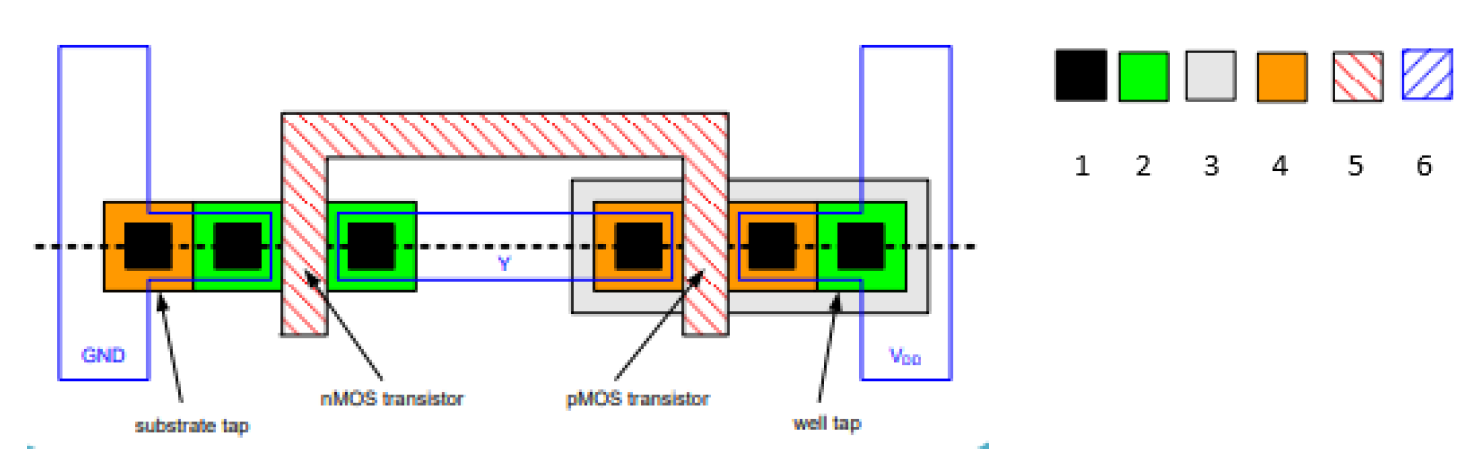
\includegraphics[width=0.8\textwidth]{inverter_layout.png}}
			\label{fig::inverter_layout}
		\end{figure}
		
		The materials in the layout are defined as follows:
		
		\begin{itemize}
			\item Material 1 (solid black) is contact material. It is made of metal (usually aluminum).
			\item Material 2 (solid green) is n+ diffusion (heavily doped n-type semiconductor [usually Si])
			\item Material 3 (solid gray) is the n-well (lightly doped n-type semiconductor [usually Si])
			\item Material 4 (solid orange) is the p+ diffusion (heavily doped p-type semiconductor [usually Si])
			\item Material 5 (striped red) is the polysilicon.
			\item Material 6 (striped blue) is the metal1 (usually aluminum)
		\end{itemize}
		
		The material layers are fabricated from the bottom up in the following order:
		
		\begin{enumerate}
			\item[1.] Material 3 (the n-well)
			\item[2.] Material 5 (polysilicon)
			\item[3.] Material 2 (n+ diffusion)
			\item[4.] Material 3 (p+ diffusion)
			\item[5.] Material 1 (contact)
			\item[6.] Material 6 (metal1)
		\end{enumerate}
	\end{enumerate}
\end{document}